% This is a LaTeX thesis template for Monash University.
% to be used with Rmarkdown
% This template was produced by Rob Hyndman
% Version: 6 September 2016

\documentclass{monashthesis}

%%%%%%%%%%%%%%%%%%%%%%%%%%%%%%%%%%%%%%%%%%%%%%%%%%%%%%%%%%%%%%%
% Add any LaTeX packages and other preamble here if required
%%%%%%%%%%%%%%%%%%%%%%%%%%%%%%%%%%%%%%%%%%%%%%%%%%%%%%%%%%%%%%%

\author{Xiefei Li}
\title{Revisiting the forecast combination puzzle: An empirical study}
\studentid{30204232}
\studentemail{\href{mailto:xlii0145@student.monash.edu}{\nolinkurl{xlii0145@student.monash.edu}}}
\studentdetails{Supervisor: David T. Frazier}
\supervisoremail{\href{mailto:David.frazier@monash.edu}{\nolinkurl{David.frazier@monash.edu}}}
\def\degreetitle{Bachelor of Commerce (Honours)}
% Add subject and keywords below
\hypersetup{
     %pdfsubject={The Subject},
     %pdfkeywords={Some Keywords},
     pdfauthor={Xiefei Li},
     pdftitle={Revisiting the forecast combination puzzle: An empirical study},
     pdfproducer={Bookdown with LaTeX}
}


\bibliography{thesisrefs}

\begin{document}

\pagenumbering{roman}

\titlepage

{\setstretch{1.2}\sf\tighttoc\doublespacing}

\clearpage\pagenumbering{arabic}\setcounter{page}{1}

\hypertarget{introduction}{%
\chapter{Introduction}\label{introduction}}

\hypertarget{research-objective}{%
\section{Research Objective}\label{research-objective}}

This thesis aims to investigate the determinants behind, and evidence for the forecast combination puzzle in various domains, and to empirically examine a general solution to the forecast combination puzzle. The combination puzzle refers to the well-known empirical finding that an equally weighted combination of forecasts generally outperforms more sophisticated combination schemes. This phenomenon is often found in the point combinations but it also appears in the density combinations. In this project, we will work with the density distribution and point forecasts are implicitly included. The use of density forecasts also offers forecasters a more comprehensive view of the target variable. Over the past 50 years, the empirical studies undertaken so far have focused more on different time series settings. Thus, one of the main contributions of this research will be to investigate the presence of the combination puzzle in settings outside of pure time series models with density forecasts. As an additional contribution, we will assess the veracity, and applicability, of a recently proposed solution to the forecast combination puzzle suggested in \textcite{ZMFP22} and \textcite{FZMP23}.

\hypertarget{literature-review-and-motivation}{%
\section{Literature Review and Motivation}\label{literature-review-and-motivation}}

The accuracy of forecasts is of critical concern for forecasters and decision makers. An idea of combining multiple forecasts from different models was originally proposed in the seminal work of \textcite{BG69}. With the evidence of dramatic improvements in the forecast accuracy, forecast combinations have attracted increasing attention and contributions in the literature, both theoretical and applied \autocite{C89,T06}. In short, forecast combination methods involve producing point or density forecasts and then combining them based on a rule or weighting scheme. This process can sometimes capture more meaningful characteristics of the true data generating process than using a single model, and allow us to combine the best features of different models within a single framework. Researchers have examined a variety of combination methods for point and density forecasts over the past 50 years, see \textcite{WHLK22} for a modern literature review.

In most time series setting under which forecast combinations are employed, a striking empirical phenomenon is often observed, coined by \textcite{SW04}, as the ``forecast combination puzzle''. The puzzle is encapsulated by the fact that ``theoretically sophisticated weighting schemes should provide more benefits than the sample average from forecast combination, while empirically the simple average has been continuously found to dominate more complicated approaches to combining forecasts'' \autocite{WHLK22}. In the literature, there are two possible explanations for the puzzle. One concentrates on the estimation uncertainty and instability in combination weight like in \textcite{SW98}, \textcite{SW04} and \textcite{SW09}. Another one explores the trade-off between bias and variance as in \textcite{E11} and \textcite{CMVW16}. Recently, \textcite{ZMFP22} and \textcite{FZMP23} proposed a new aspect of explanation by investigating the sampling variability in model estimation. They illustrated that, asymptotically, the bias and variability mainly come from the estimation of forecasts.

The goal of this thesis is two-fold: first, to search for empirical evidence of the combination puzzle in settings outside of the usual time series in which it has been found; second, to test the empirical veracity of the theoretical solution to the puzzle found in \textcite{FZMP23}, both within, and outside of, the standard time series setting where the puzzle is often observed.

\hypertarget{methodology}{%
\chapter{Methodology}\label{methodology}}

The first goal of this paper is to construct linear density forecast combinations with parametric models. The results are anticipated to reveal that forecast combinations can deliver improved accuracy over single models, but are not necessarily superior to forecasts obtained from the equally weighted combination.

The next goal is to estimate the unknown parameters of the constituent models and the weight in a single step, and to compare the accuracy of forecasts based on these combinations against the usual combinations process, as well as the equally weighted combination. To measure differences between these forecasts, we will eventually employ forecast accuracy tests, of the type derived in \textcite{W96}, which measure out-of-sample differences between forecasts.

Before explaining the details, the following notations will be used throughout the paper. A vector time series \(\textbf{y}_t\) with a total of \(T\) observations will be divided proportionally into two parts, an in-sample period \(R\) and an out-of-sample period \(P\). The realization of a target variable \(y\) at time \(t\) is denoted as \(y_{t}\). Its future value after the in-sample period is denoted as \(y_{\small{R+h}}\), where \(h\) is the forecast horizon and \(h>0\). The information set at time t, \(\mathcal{F}_t\), is comprised of all observed (and known) realizations of \(y\) up to time t, i.e., \(\mathcal{F}_t = \{y_1, y_2, .., y_t\}\).

A prediction model \(M\) determines the conditional probability density for \(\textbf{y}_t\) with unknown parameters \(\theta_M\) given the history \(\mathcal{F}_{t-1}\), denoted by \(f(y_t|\mathcal{F}_{t-1}, \theta_M, M)\). Parameter estimates \(\hat\theta_M\) are obtained by maximizing the log likelihood function of the conditional probability density for the in-sample period, i.e., \(\hat\theta_M = \text{argmax} \sum^R_{t=1} log f(y_t|\mathcal{F}_{t-1}, M)\). These estimates will be held fixed for the easy of evaluation.

\hypertarget{forecast-combination-method}{%
\section{Forecast Combination Method}\label{forecast-combination-method}}

Based on the idea of linear pooling \autocite{BG69,HM07,GA11}, a linear combination of two predictive densities \(f^{(t)}\) is constructed with two constituent predictive densities \(f^{(t)}_1\) and \(f^{(t)}_2\):

\begin{equation}
f^{(t)}(y) = wf^{(t)}_1(y) + (1-w)f^{(t)}_2(y)
\end{equation}

where \(h\) is the future value after the in-sample period (\(R\)), and \(w\) is the weight allocated to the first model. Through this construction, the sum of two weights is implied to be 1, which is necessary and sufficient for the combination to be a density function \autocite{GA11}.

Following the literature on density forecast evaluation, our initial analysis will focus on using log predictive score functions to assess the model estimation and measure the accuracy of our density forecasts; see, e.g., \textcite{GA11} for a discussion on log score and its use in density forecasting. The log predictive score function of a specific model over the forecast horizon \(h=1,2,...,P\) (i.e., the out-of-sample period) is defined as follows:

\begin{equation}
LS = \sum^P_{h=1} logf(y_{\small{R+h}}| \mathcal{F}_{\small{R+h-1}})
\end{equation}

The weight \(w\) assigned to the first model will be estimated by maximizing the log predictive score function over the out-of-sample period:

\begin{equation}
\sum^P_{h=1}log\Big[wf_1(y_{\small{R+h}}|\mathcal{F}_{\small{R+h-1}}) + (1-w)f_2(y_{\small{R+h}}|\mathcal{F}_{\small{R+h-1}})\Big]
\end{equation}

\hypertarget{preliminary-results}{%
\chapter{Preliminary Results}\label{preliminary-results}}

\hypertarget{a-motivating-example}{%
\section{A Motivating Example}\label{a-motivating-example}}

Reconsidering the example in section 3 of \textcite{GA11}, the data used is the daily Standard and Poor's (S\&P) 500 index from February 11, 2013 to February 10, 2023 (10 years in total), retrieved via the \textcite{SP500}. We choose \(j=1,\cdots,M\), with \(M=5\) prediction models to study the performance of density predictions across sets of \texttt{two-model} pools. Each of the \(j\) predictive model has a conditionally Gaussian density, which takes the form \(f^{(j)}(y)=f_j(y_t|\mathcal{F}_{t-1})=N\{y_t; \mu_j, \sigma^2_j\}\), where \(N\{x; \mu, \sigma^2\}\) denotes the normal probability density function evaluated at value \(x\) with mean \(\mu\) and variance \(\sigma^2\). The notation \(\mathcal{F}_{t-1}\) denotes all information available at time \(t-1\), and we assume that the conditional mean and variance of the models are, up to unknown parameters, known at time \(t-1\).

Models include commonly used model types such as autoregressive integrated moving average (ARIMA), exponential smoothing (ETS), and linear regression model with ARIMA errors. See Appendix for detailed model specifications.

There are 10 sets of two-model combination and each combination log score is generated according to (2.3) with the value of weight changes by 0.01 every time. Table \ref{tab:2} shows the estimated weights and combination log scores.

\begin{table}[ht]
  \centering
  \caption{Log predictive score of density forecasts combination under two-model pools}
    \begin{tabular}{llllll}
    \toprule
          & ARIMA(1,1,1) & ETS(M,N,N) & ETS(M,A,N) &  LM (linear) &  LM (log) \\
    \midrule
    ARIMA(1,1,1) & \textit{-5911.1974} & -5839.3045 & -5842.7634 & -5911.1974 & -5894.1267 \\
    ETS(M,N,N) & 0.45  & \textit{-5883.9697} & -5881.7790 & -5883.9697 & -5858.6397 \\
    ETS(M,A,N) & 0.43  & 0.08  & \textit{-5881.7970} & -5881.7970 & -5859.7980 \\
     LM (linear) & 1     & 1     & 1     & \textit{-7532.1464} & -5918.5230 \\
     LM (log) & 0.56  & 0.65  & 0.67  & 0     & \textit{-5918.5230} \\
    \bottomrule
    \multicolumn{6}{l}{\footnotesize The diagonal entries contains individual log score.}\\
    \multicolumn{6}{l}{\footnotesize The log scores for combination pools are located above the diagonal.}\\
    \multicolumn{6}{l}{\footnotesize Entries below the diagonal show the estimated weight of the model in that column in the two-model pool.}\\
    \end{tabular}
  \label{tab:2}
\end{table}

\vspace{0.3cm}

\begin{figure}[ht]
\centering
\caption{The highest four log predictive scores of weighted two-model-pool combinations for S\&P 500 returns predictive densities. }
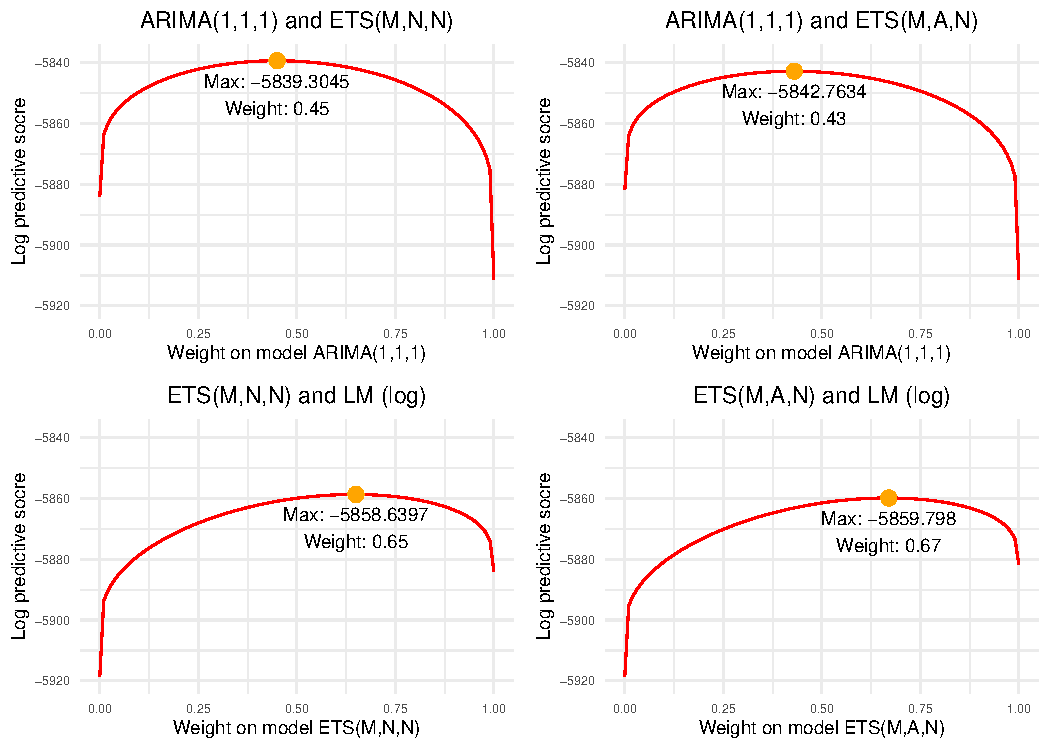
\includegraphics{figures/best4comb.pdf}
\begin{flushleft}
{\footnotesize The weights on the first model is in the x-axis and the corresponding log predictive scores are on the y-axis. Constitutent models are stated in the title. The orange point represent the highest log score of a specific combination. Its value and the corresponding optimal weight are noted below.}\\
\end{flushleft}
\label{fig:best4}
\end{figure}

Figure \ref{fig:best4} illustrates the change of the log predictive score for the top 4 combinations as the weight increases. The great improvement in the scores means that the combination forecasts do perform better than the individual forecasts. It is also noticeable that the estimated weights are close to the equal weight (0.5), which could be an evidence for the forecast combination puzzle.

\hypertarget{timeline-of-future-research}{%
\section{Timeline of Future Research}\label{timeline-of-future-research}}

\begin{table}[htbp]
  \centering
  \caption{Research Plan}
    \begin{tabular}{ll}
    Time  & Objectives \\
    \midrule
    May - June & Investigating the presence of puzzle in panel data and literature review \\
    July - August & Applying the forecast accuracy tests with time series data and drafting thesis  \\
    September & Attempting the tests with panel data and considering limitations \\
    October & Working on thesis and final presentation \\
    \end{tabular}
\end{table}

\appendix

\hypertarget{appendix}{%
\chapter{Appendix}\label{appendix}}

The S\&P500 returns dataset has a total of 2519 (\(T\)) observations and is partitioned into two periods with a rough proportion. The in-sample period contains the first 60\% of the data (\(R = 1511\)), which is used for estimating unknown parameters in each model. The remaining 40\% (\(P = 1008\)) becomes the out-of-sample period for further evaluation.

The following prediction models are used to study the performance of two-model pools:

\begin{enumerate}
\def\labelenumi{\arabic{enumi}.}
\tightlist
\item
  Model 1: An ARIMA(1,1,1) model with an intercept for the natural logarithm of S\&P 500.
\item
  Model 2: An ETS(M,N,N) model for the S\&P 500.
\item
  Model 3: An ETS(M,A,N) model for the S\&P 500.
\end{enumerate}

All error terms are assumed to be independent and normally distributed with mean zero and variance \(\sigma_j^2 \ \text{for}\  j = 1,2,3\).

\begin{enumerate}
\def\labelenumi{\arabic{enumi}.}
\setcounter{enumi}{3}
\tightlist
\item
  Model 4: A linear regression model for the S\&P 500 with a trend regressor and errors, follow an ARIMA(1,0,0) process.
\item
  Model 5: A linear regression model for the natural logarithm of S\&P 500 with a trend regressor and errors follow an ARIMA(1,0,0) process.
\end{enumerate}

Both error terms in the ARIMA model are assumed to be independent and normally distributed with mean zero and variance \(\sigma_j^2 \ \text{for}\  j = 4,5\).

Exact formulas and explanations of these models can be found in \textcite{fpp3}. The formula of the conditional variance for the ETS models in this case is discussed in Chapter 6.3 of \textcite{HKOS08}. All coding is performed using R Statistical Software (version 4.2.1 (2022-06-23)). The packages used are \texttt{tidyverse} \autocite{tidy19}, \texttt{dplyr} \autocite{dplyr23}, and \texttt{fpp3} \autocite{fpp23}.

All unknown parameters are estimated by maximizing the likelihood function using the in-sample period data. Once the estimated are obtained, they are held fixed for the density evaluation. For each model, we generate the predictive densities at every future time point of S\&P 500 returns (\(h=1,2,...,P\)) given that all past information is known. In order to make a comparison between models, the log of S\&P 500 returns will be evaluated by the log normal density function.

The log predictive score of each model is calculated and presented in Table \ref{tab:1}. If only one model can be chosen, the model with the highest score will be preferred, which is the ETS(M,A,N) model with a score of -5881.7970 in this case.

\vspace{0.3cm}

\begin{table}[htbp!]
\centering
\caption{Log predictive score of each proposed model for S\&P 500 returns.}
\begin{tabular}{l*{4}{c}cccccccc}
\hline
     ARIMA(1,1,1) & ETS(M,N,N) & ETS(M,A,N) & LM (linear) & LM (log) \\
    \hline
     -5911.1974 & -5883.9697  & -5881.7970 & -7532.1464 & -5918.5230\\
    \hline
\end{tabular}
\label{tab:1}
\end{table}

The top 4 combinations and their log scores are collected in Table \ref{tab:3}.

\begin{table}[ht]
  \centering
  \caption{The top four density forecasts combinations evaluated by the log predictive score}
    \begin{tabular}{ll}
    \toprule
    Combination & Log predictive score \\
    \midrule
    ARIMA(1,1,1) \& ETS(M,N,N) & -5839.3045 \\
    ARIMA(1,1,1) \& ETS(M,A,N) & -5842.7634 \\
    ETS(M,N,N) \&  LM (log) & -5858.6397 \\
    ETS(M,A,N) \&  LM (log) & -5859.7980 \\
    \bottomrule
    \end{tabular}
  \label{tab:3}
\end{table}

\printbibliography[title={Reference}]




\end{document}
